% !TEX root = C:\Users\panen\ex.tex
\documentclass[14pt,a4paper]{scrartcl}
\usepackage[utf8]{inputenc}
\usepackage{ragged2e}
\usepackage[english,russian]{babel}
\usepackage{misccorr,color,ragged2e,amsfonts,amsthm,graphicx,systeme,amsmath,mdframed,lipsum}
\usepackage{tikz}
\usepackage{esvect}
\usepackage{graphicx}
\usepackage{slashbox}
\usepackage{diagbox}
\usepackage{float}
\usepackage{comment}
\usepackage{amsmath}
\usepackage{alltt}
\usepackage{ amssymb }
\usepackage[unicode]{hyperref}
%\graphicspath{ {C:\Users\panen\CW_1_Probalility} }
\renewcommand\qedsymbol{$\blacksquare$}
\renewcommand*{\proofname}{\text{Доведення}}
\theoremstyle{definition}
\newtheorem{defo}{Означення}[section]
\newtheorem*{teo}{Теорема}
\newtheorem*{example}{Приклад}
\theoremstyle{remark}
\newtheorem*{remark}{Зауваження}
\theoremstyle{definition}
\newtheorem*{consequence}{Наслідок}
\theoremstyle{definition}
\newtheorem{statement}{Утверждение}[section]
\newmdtheoremenv{boxteo}{Теорема}[section]
%\setlength\parindent{0pt}
\usepackage{lipsum}
\setlength{\parindent}{5ex}
\DeclareMathOperator*\lowlim{\underline{lim}}
\DeclareMathOperator*\uplim{\overline{lim}}
\setcounter{subsection}{-1}
\usepackage{tabularx}


% Default fixed font does not support bold face
\DeclareFixedFont{\ttb}{T1}{txtt}{bx}{n}{12} % for bold
\DeclareFixedFont{\ttm}{T1}{txtt}{m}{n}{12}  % for normal

% Custom colors
\usepackage{color}
\definecolor{deepblue}{rgb}{0,0,0.5}
\definecolor{deepred}{rgb}{0.6,0,0}
\definecolor{deepgreen}{rgb}{0,0.5,0}

\usepackage{listings}

% Python style for highlighting
\newcommand\pythonstyle{\lstset{
language=Python,
basicstyle=\ttm,
otherkeywords={self},             % Add keywords here
keywordstyle=\ttb\color{deepblue},
emph={MyClass,__init__},          % Custom highlighting
emphstyle=\ttb\color{deepred},    % Custom highlighting style
stringstyle=\color{deepgreen},
frame=tb,                         % Any extra options here
showstringspaces=false            %
}}

\definecolor{javared}{rgb}{0.6,0,0} % for strings
\definecolor{javagreen}{rgb}{0.25,0.5,0.35} % comments
\definecolor{javapurple}{rgb}{0.5,0,0.35} % keywords
\definecolor{javadocblue}{rgb}{0.25,0.35,0.75} % javadoc

\lstset{language=C++,
basicstyle=\ttfamily,
keywordstyle=\color{javapurple}\bfseries,
stringstyle=\color{javared},
commentstyle=\color{javagreen},
morecomment=[s][\color{javadocblue}]{/**}{*/},
numbers=left,
numberstyle=\tiny\color{black},
stepnumber=2,
numbersep=10pt,
tabsize=4,
showspaces=false,
showstringspaces=false}


% Python environment
\lstnewenvironment{python}[1][]
{
\pythonstyle
\lstset{#1}
}
{}

% Python for external files
\newcommand\pythonexternal[2][]{{
\pythonstyle
\lstinputlisting[#1]{#2}}}

% Python for inline
\newcommand\pythoninline[1]{{\pythonstyle\lstinline!#1!}}
%
% \begin{python}
% class MyClass(Yourclass):
%     def __init__(self, my, yours):
%         bla = '5 1 2 3 4'
%         print bla
% \end{python}

\begin{document}

\begin{titlepage}
    \newpage
    \begin{center}
    {\bfseries Национальный технический университет Украины «Киевский политехнический институт имени Игоря Сикорского»}
    \vspace{1cm}
    %САНКТ-ПЕТЕРБУРГСКИЙ \\*
    %ГОСУДАРСТВЕННЫЙ УНИВЕРСИТЕТ \\*
    %\hrulefill
    %\end{center}

    %{КАФЕДРА ЯДЕРНОЙ ФИЗИКИ }
    Кафедра Математических Методов Системного Анализа
    \vspace{6em}



    %\vspace{2.0em}

    %\begin{center}
     %AndreyOlegovich.ru \\
    \end{center}

    \vspace{1.2em}

    \begin{center}
    %\textsc{\textbf{}}
    \Large Расчетная работа с дисциплины "Математическая статистика"
    \end{center}

    \vspace{5em}

    \begin{center}
    %\Large
     %Панченко Егор
     \end{center}
    \vspace{6em}

    %\begin{center}
    %\begin{tabbing}
    %\begin{center}
    %\quad\=Научный руководитель \\
    %\>д.ф.м.н., Andrey В.А.\\
    %\vspace{1.2em}
    %\>Рецензент \\
    %\>к.ф.-м.н. Olegovich В.И.\\
    %\end{tabbing}
    %\end{center}

    \begin{alltt}
                       Проверил
                       к.ф.м.н. Каниовская И. Ю.
                       Выполнил
                       студент и просто хороший человек Панченко Е. С.
    \end{alltt}


    \vspace{\fill}

    \begin{center}
    Киев 2021
    \end{center}

    \end{titlepage}

\tableofcontents
\newpage

\def\be{\begin{equation}}
\def\ee{\end{equation}}
\def\bd{\begin{defo}}
\def\ed{\end{defo}}
\def\bbt{\begin{boxteo}}
\def\ebt{\end{boxteo}}
%\begin{comment}
\section{Постановка задачи}

Задана выборка

\begin{align*}
  \begin{tabularx}{\textwidth}{| X | X | X | X | X | X | X | X | X | X |}
  \hline
    $2$ & $1$ & $3$ & $1$ & $0$ & $1$ & $3$ & $2$ & $2$ & $2$ \\ \hline
    $4$ & $5$ & $1$ & $3$ & $2$ & $2$ & $2$ & $4$ & $2$ & $2$ \\ \hline
    $4$ & $5$ & $6$ & $4$ & $3$ & $5$ & $2$ & $4$ & $2$ & $4$ \\ \hline
    $3$ & $3$ & $5$ & $9$ & $6$ & $3$ & $5$ & $7$ & $1$ & $6$ \\ \hline
    $3$ & $2$ & $1$ & $4$ & $9$ & $5$ & $4$ & $5$ & $4$ & $5$ \\ \hline
    $4$ & $4$ & $9$ & $2$ & $1$ & $6$ & $1$ & $5$ & $3$ & $5$ \\ \hline
    $5$ & $3$ & $6$ & $9$ & $3$ & $6$ & $4$ & $4$ & $4$ & $8$ \\ \hline
    $3$ & $7$ & $4$ & $5$ & $2$ & $6$ & $4$ & $3$ & $3$ & $3$ \\ \hline
    $4$ & $2$ & $4$ & $2$ & $3$ & $5$ & $4$ & $3$ & $4$ & $5$ \\ \hline
    $2$ & $2$ & $6$ & $3$ & $5$ & $2$ & $6$ & $2$ & $1$ & $1$ \\ \hline
  \end{tabularx}
\end{align*}

Основная цель - найти, каким распределением она порождена и аргументировать, почему.

\section{Решение задачи}

\subsection{Построение вариационного ряда данной выборки}
Поскольку в выборке содержатся только целые числа и большинство из них не уникально, то автор решил построить дискретный ряд. Для этого строится табличка, которая по каждой варианте показывет ее частость и частотность.
\begin{align*}
  \begin{tabular}{ | l | l | l | l | l | l | l | l | l | l | l |}
  \hline
    варианты & $0$ & $1$ & $2$ & $3$ & $4$ & $5$ & $6$ & $7$ & $8$ & $9$ \\ \hline
    частоты $n_i$ & 1 & 10 & 20 & 18 & 20 & 15 & 9 & 2 & 1 & 4 \\ \hline
    частотности $w_i$ & 0.01 & 0.1 & 0.2 & 0.18 & 0.2 & 0.15 & 0.09 & 0.02 & 0.01 & 0.04 \\ \hline
  \end{tabular}
\end{align*}

\subsection{Графическое изображение выборки}
Изображение выборки было решено представить в виде гистограммы, где каждый столбец представляет собой варианту, а высота каждого столбца - ее частость. Гистограмма имеет вид:
\begin{figure}[H]
  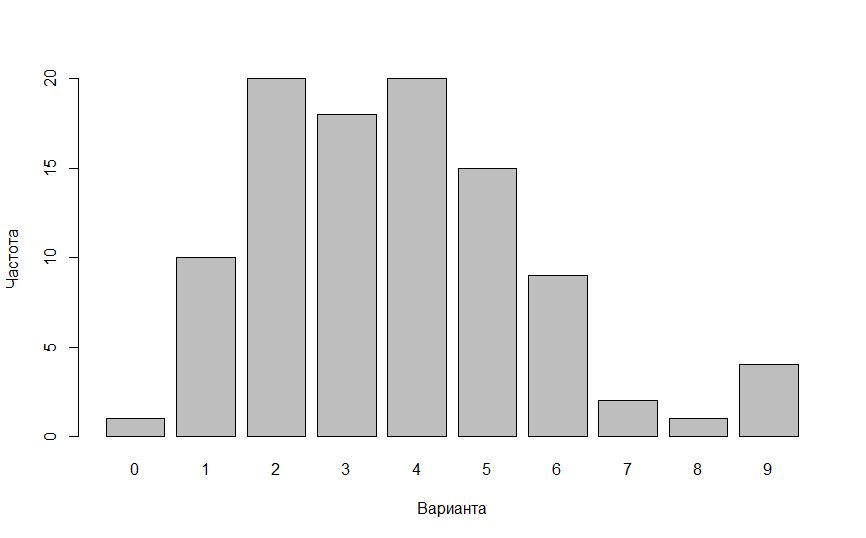
\includegraphics[width=\linewidth]{Plot1.png}
  \caption{Гистограмма выборки}
  \label{fig:image1}
\end{figure}

\subsection{Эмпирическая функция распределения}
Построим эмпирическую функцию распределения:
\begin{align*}
  F_{100}^{*}(x) = \begin{cases}
    0,  & \mbox{если } x\leq0; \\
    0.01, & \mbox{если } 0<x\leq1; \\
    0.01+0.1=0.11, & \mbox{если } 1<x\leq2; \\
    0.01+0.1+0.2=0.31, & \mbox{если } 2<x\leq3; \\
    0.01+0.1+0.2+0.18=0.49, & \mbox{если } 3<x\leq4; \\
    0.01+0.1+0.2+0.18+0.2=0.69, & \mbox{если } 4<x\leq5; \\
    0.01+0.1+0.2+0.18+0.2+\\+0.15=0.84, & \mbox{если } 5<x\leq6; \\
    0.01+0.1+0.2+0.18+0.2+\\+0.15+0.09=0.93, & \mbox{если } 6<x\leq7; \\
    0.01+0.1+0.2+0.18+0.2+\\+0.15+0.09+0.02=0.95, & \mbox{если } 7<x\leq8; \\
    0.01+0.1+0.2+0.18+0.2+\\+0.15+0.09+0.02+0.01=0.96, & \mbox{если } 8<x\leq9; \\
    0.01+0.1+0.2+0.18+0.2+\\+0.15+0.09+0.02+0.01+0.04=1, & \mbox{если } x>9. \\
  \end{cases}
\end{align*}
Убрав промежуточные расчеты, получим
\begin{align*}
  F_{100}^{*}(x) = \begin{cases}
    0,  & \mbox{если } x\leq0; \\
    0.01, & \mbox{если } 0<x\leq1; \\
    0.11, & \mbox{если } 1<x\leq2; \\
    0.31, & \mbox{если } 2<x\leq3; \\
    0.49, & \mbox{если } 3<x\leq4; \\
    0.69, & \mbox{если } 4<x\leq5; \\
    0.84, & \mbox{если } 5<x\leq6; \\
    0.93, & \mbox{если } 6<x\leq7; \\
    0.95, & \mbox{если } 7<x\leq8; \\
    0.96, & \mbox{если } 8<x\leq9; \\
    1, & \mbox{если } x>9. \\
  \end{cases}
\end{align*}

Ниже приводится график эмпирической функции распределения.

\begin{figure}[H]
  \includegraphics[width=\linewidth]{RPlotDistrFunc1.png}
  \caption{График эмпирической функции распределения}
  \label{fig:image4}
\end{figure}

\subsection{Выборочные медиана, мода и ассиметрия}
Выборочная медиана есть медиана выборки. То есть для ее вычисления достаточно взять среднее арифметическое 50-го и 51-го элементов, когда выборка предварительно упорядочена:
\begin{align*}
  Me^{*}(\xi) = \frac{4 + 4}{2} = 4.
\end{align*}
Выборочной модой есть те варианты, которые в выборке встречаются наибольшее число раз. В данной выборке есть две варианты, которые встречаются чаще других - это 2 и 4. То есть
\begin{align*}
  Mo^{*}(\xi) = \{2, 4\}.
\end{align*}
Выборочная ассиметрия считается по формуле
\begin{align*}
  As^{*}(\xi) = \frac{\frac{1}{n}\sum_{i = 1}^{n} (\xi_i - \overline{\xi})^{3}}{(\mathbb{D}^{*}\xi)^{3/2}},
\end{align*}
где $\overline{\xi}$ - выборочное среднее и $\mathbb{D}^{*}\xi$ - выборочная диспресия.
Считаем значения выборного среднего и выборочной дисперсии на данной выборке:
\begin{align*}
  &\overline{x} = \frac{1}{n} \sum_{i = 1}^{100} x_i = 3.71,\\
  &(\mathbb{D}^{*} \xi)_{val} = \frac{1}{n} \sum_{i = 1}^{100} (x_i - \overline{x})^2 = 3.844343, \\
  &(As^{*} \xi)_{val} = \frac{\frac{1}{100}\sum_{i = 1}^{100} (x_i - 3.71)^{3}}{(3.844343)^{3/2}} \approxeq 0.709.
\end{align*}

\subsection{Нахождение несмещенных оценок математического ожидания и дисперсии}

Известно, что исправленная выборочная дисперсия - это несмещенная оценка дисперсии генеральной совокупности. В дальнейшей работе этого факта нам будет вполне достаточно. Подробно про несмещенную оценку математического ожидания будет написано в седьмом подзаголовке.

\subsection{Выдвижение гипотезы про распределение, за которым получено выборку}

Мое предположение, что выборка порождена распределением Пуассона. Для этого есть несколько причин. Самое главное замечание, что в выборке содержаться только целые числа. Из этого я делаю вывод, что распределение, скорее всего, дискретное. Геометрическое вряд-ли, потому что столбцы в гистограмме не убывают. Есть вариант, что это может быть и биномиальное распределение. Сначала я проверю, порождена ли эта выборка распределением Пуассона, и если нет, то перейду на биномиальное рапсределение. Также я поигрался с разными значениями параметров для распределения Пуассона и биномиального распределения. Ниже можно увидеть ряд графиков, которые подтверждают обе мои гипотезы.

\begin{figure}[H]
  \includegraphics[width=\linewidth]{RPlotPoiss.png}
  \caption{Случайно сгенерированные выборки, попрожденные законом Пуассона с параметром $a = 3.71$}
  \label{fig:image2}
\end{figure}

\begin{figure}[H]
  \includegraphics[width=\linewidth]{RPlotBinom.png}
  \caption{Случайно сгенерированные выборки, порожденные биномиальным законом с параметрами $size = 20, p = 0.2$}
  \label{fig:image3}
\end{figure}

\subsection{Нахождение точковых оценок параметров распределения Пуассона и проверить их свойства}

Пусть наша выборка порождена распределением Пуассона, то есть
\begin{align*}
  \xi \sim Poiss(a).
\end{align*}

Известно, что математическое ожидание случайной величины, распределенной по распределению Пуассона с параметром $a$, есть само число $a$. Исходя из этого, выберем в качестве точечной оценки параметра $a$ выборочное среднее.
Исследуем свойства этой точечной оценки. Известно, что выборочное среднее есть несмещенной оценкой математического ожидания, а также эта оценка есть конзистентной. Проверим ее эффективность:

\begin{align*}
  &ln \mathcal{L}(\vec{x}, a) = -n\cdot a + ln(a)\cdot \sum_{i = 1}^{n} x_i - \sum_{i = 1}^{n} ln(x_i!), \\
  &\frac{\partial ln \mathcal{L}(\vec{x}, a)}{\partial a} = -n + \frac{1}{a}\cdot \sum_{i = 1}^{n} x_i = \frac{n}{a}\cdot (\overline{x} - a).
\end{align*}

Поскольку множитель перед $(\overline{x} - a)$ зависит только от $n$ и от $a$, то оценка является эффективной.

Подытожим: на данный момент у нас есть несмещенная, конзистентная и эффективная оценка параметра гипотетического закона распределения. Это уже неплохой старт. Найдем теперь точечную оценку параметра $a$ двумя методами - методов моментов и методом максимальной правдоподобности.

\subsubsection{Метод моментов}

Суть метода моментов в том, что эмпирические моменты приравниваются к теоретическим моментам. Если из этих равенств можно вытянуть числовое значение некой характеристики, то это значение можно брать за значение точечной оценки этой характеристики. К делу, приравняем моменты первых порядков:

\begin{align*}
  a^{*} = E\xi = E^{*}\xi = \overline{\xi}.
\end{align*}

Получили, что $a_{\text{ММ}}^{*} = \overline{x} = 3.71.$

\subsubsection{Метод максимальной правдоподобности}

Суть метода максимальной правдоподобности в том, чтобы максимизировать значение функции правдоподобности. Функция правдоподобности распределения Пуассона есть

\begin{align*}
  ln \mathcal{L}(\vec{x}, a) = -n\cdot a + ln(a)\cdot \sum_{i = 1}^{n} x_i - \sum_{i = 1}^{n} ln(x_i!).
\end{align*}

Найдем критические точки:

\begin{align*}
  &\frac{\partial ln \mathcal{L}(\vec{x}, a)}{\partial a} = -n + \frac{1}{a}\cdot \sum_{i = 1}^{n} x_i = \frac{n}{a}\cdot (\overline{x} - a) = 0 \iff a_{cr} = \overline{x}.
\end{align*}

Чтобы проверить, что в точке $a_{cr}$ достигается максимум, устремим в функции правдоподобности аргумент $a$ к плюс бесконечности и к нулю. Тогда функция правдоподобности будет стремится к минус бесконечности в обоих случаях. А это значит, что в точке $a_{cr}$ достигается максимум.

Получили, что $a_{\text{ММП}}^{*} = \overline{x} = 3.71.$


\subsection{Проверка гипотезы про распределение с помощью критерия Пирсона}

Пусть некая случайная величина распределена по закону Пуассона. Построим табличку, в которой будут хранится значения вероятностей, что эта случайная величина набыла одно из значений от нуля до девяти. Округлим вероятности до четырех знаков после запятой.

\begin{align*}
  \begin{tabular}{ | l | l | l | l | l | l | l | l | l | l | l |}
  \hline
    значение случ. вел. & $0$ & $1$ & $2$ & $3$ & $4$ \\ \hline
    вероятность & 0.0244 & 0.0908 & 0.1684 & 0.2083 & 0.1932 \\ \hline
    значение случ. вел. & $5$ & $6$ & $7$ & $8$ & $9$ \\ \hline
    вероятность & 0.1433 & 0.0886 & 0.0470 & 0.0218 & 0.0089 \\ \hline
  \end{tabular}
\end{align*}

Поскольку из-за округления сумма вероятностей не равна единице, то подгоним значения вероятностей таким образом, чтобы их сумма стала единицей. Для этого сначала подсчитаем сумму всех этих вероятностей:

\begin{align*}
  sum_{prob} = 0.9947 \text{ , а заодно и } \frac{1}{sum_{prob}} \approxeq 1.005.
\end{align*}

Затем умножим каждое из чисел на на величину, обратную найденной суммы. Получим табличку

\begin{align*}
  \begin{tabular}{ | l | l | l | l | l | l |}
  \hline
    значение случ. вел. & $0$ & $1$ & $2$ & $3$ & $4$ \\ \hline
    вероятность & 0.0247 & 0.0912 & 0.1692 & 0.2093 & 0.1943 \\ \hline
    значение случ. вел. & $5$ & $6$ & $7$ & $8$ & $9$ \\ \hline
    вероятность & 0.1441 & 0.0891 & 0.0472 & 0.0219 & 0.009 \\ \hline
  \end{tabular}
\end{align*}

Теперь умножим каждую из вероятностей на размер выборки, то есть на сотню.

\begin{align*}
  \begin{tabular}{ | l | l | l | l | l | l |}
  \hline
    значение случ. вел. & $0$ & $1$ & $2$ & $3$ & $4$ \\ \hline
    $n\cdot p$ & 2.47 & 9.12 & 16.92 & 20.93 & 19.43 \\ \hline
    значение случ. вел. & $5$ & $6$ & $7$ & $8$ & $9$ \\ \hline
    $n\cdot p$ & 14.41 & 8.91 & 4.72 & 2.19 & 0.9 \\ \hline
  \end{tabular}
\end{align*}

Объясним, что сейчас будет происходить. Мы собираемся воспользоваться критерием Пирсона. Для этого мы вводим нулевую гипотезу $H_{0}$ - выборка порождена распределением Пуассона с параметром $3.71$. Наша цель показать, что гипотеза $H_{0}$ выполняется. В таком случае роботу можно оканчивать, и не проверять биномиальное распределение.

По алгоритму проверки гипотезы по критерию Пирсона, необходимо разбить множество возможных значений случайной величины на несколько непересекающихся классов. Поскольку случайная величина набывает десяти значений, то начальное число классов равно десяти. Наша цель - объеденить некоторые классы так, чтобы в каждом из классов величина $n\cdot p$ была не меньше десяти. Для этого объеденим первые два класса и последние четыре. Перепишем нашу табличку, а также внесем в нее дополнительные строки - частоты на множествах значений случайной величины, и разницы соответствующих значений.

\begin{align*}
  \begin{tabular}{ | l | l | l | l | l | l | l |}
  \hline
    значение случ. вел. $\xi_{i}$ & $\{0, 1\}$ & $2$ & $3$ & $4$ & $5$ & $\{6, 7, 8, 9\}$ \\ \hline
    $n\cdot p_{i}$ & 11.59 & 16.92 & 20.93 & 19.43 & 14.41 & 16.72\\ \hline
    частота $n_{i}$ & 11 & 20 & 18 & 20 & 15 & 16\\ \hline
    разница $n_{i} - n\cdot p_{i}$ & -0.59 & 1.08 & -0.93 & 0.57 & 0.59 & -0.72\\ \hline
  \end{tabular}
\end{align*}

Теперь необходимо подсчитать $\eta_{val}$. По определению

\begin{align*}
  \eta = \sum_{i=1}^{r} \frac{(n_{i} - n\cdot p_{i})^2}{n\cdot p_{i}}.
\end{align*}

Подставляя числа из таблицы, получим

\begin{align*}
  \eta_{val} = \frac{(-0.59)^2}{11.59} + \frac{(1.08)^2}{16.92} + \frac{(-0.93)^2}{20.93} + \frac{(0.57)^2}{19.43} + \frac{(0.59)^2}{14.41} + \frac{(-0.72)^2}{16.72} \approxeq 0.2121.
\end{align*}

По теореме Пирсона статистика $\eta$ стремится по распределению к распределению $\chi_{r-s-1}^2$, где $r$ - число классов, а $s$ - число неизвестных параметров. В нешем случае $r = 6$ и $s = 1$. Смотрим в таблицу квантилей распределения Пирсона, и находим, что $t_{cr} = 9.49.$

Поскольку $\eta_{val} < t_{cr}$, то можно порадоваться, ведь наши данные не противоречат выдвинутой гипотезе $H_{0}$.

\subsection{Нахождения доверительного интервала гипотетического закона распределения}

По центральной граничной теореме, приблизительно имеем, что

\begin{align*}
  \overline{\xi} \sim N(E\xi, \frac{D\xi}{n}).
\end{align*}

Или

\begin{align*}
  \overline{\xi} \sim N(a, \frac{a}{n}).
\end{align*}

Или, нормируя случайную величину:

\begin{align*}
  \eta = \frac{(\overline{\xi}-a)\cdot \sqrt{n}}{\sqrt{a}} \sim N(0, 1).
\end{align*}

Задача нахождения доверительного интервала состоит в том, чтобы отыскать такие числа $t_{1}$ и $t_{2}$, чтобы $P\{t_{1} < a < t_{2}\}$ была не менее $\gamma$. По условию $\gamma = 0.95$. Для упрощения задачи будем искать именно симметричный интервал относительно точки $a$. Тогда наша вероятность перепишется в виде

\begin{align*}
  P\{|\eta| < t_{\gamma}\} = \gamma,
\end{align*}

где $t_{\gamma}$ находится из таблицы Лапласса. Поскольку

\begin{align*}
  P\{|\eta| < \varepsilon\} = 2 \cdot \text{Ф}(\varepsilon) = \gamma = 0.95, \text{ откуда } \varepsilon = t_{\gamma} = 1.96.
\end{align*}

Запишем цепочку преобразований

\begin{align*}
  &|\eta| < 1.96 \iff \frac{|\overline{\xi}-a|\cdot \sqrt{n}}{\sqrt{a}} < 1.96 \iff \\
  &\frac{|3.71-a|\cdot 10}{\sqrt{a}} < 1.96 \iff (3.71-a)^2 \cdot 100 < 1.96^2 \cdot a \iff \\
  &a^2-7.42\cdot a + 13.7641 < 0.038416\cdot a \iff 3.3512 < a < 4.10722.
\end{align*}

То есть доверительный интервал есть $(3.3512, 4.10722).$

\subsection{Выводы}

\end{document}
